\section{Amplitude Modulation:Single Sideband(SSB)}

The DSB spectrum has two sidebands: the upper sideband(USB) and the lower sideband(LSB),both containing the complete information of the baseband signal.A scheme in which only one sideband is transmitted is known as \textbf{single side-band(SSB) transmission},which requires only one-half the bandwidth of the DSB signal.
An SSB signal can be coherently(synchronously) demodulated.For example, multiplication of a USB signal by $\cos\omega_ct$ shifts its spectrum to the left and write by $\omega_c$.The case is similar with the LSB signals.Hence the demodulation of SSB signal is identical to that of DSB-SC signals.

\begin{figure}[H]
  \centering
  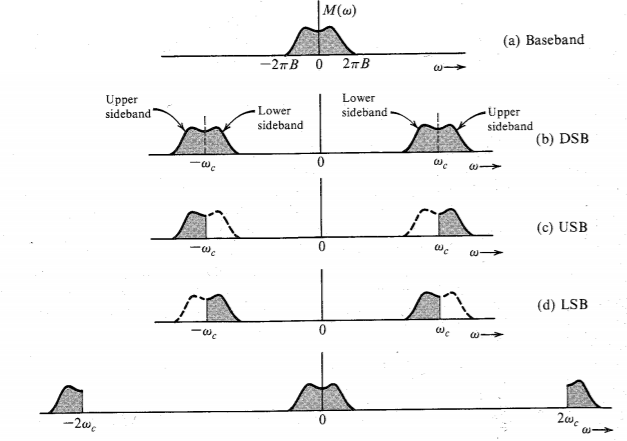
\includegraphics[]{Capture1.PNG}
  \caption{SSB Spectra}
\end{figure}

\subsection{Time Domain Representation of SSB Signals}
Because the building block of an SSB signal are the sidebands, we shall first obtain a time domain expression for each sideband. Figure 2 shows the spectrum M($\omega$).The USB and LSB are also shown there.From the figure we can obtain that $M_+(\omega)$=$M(\omega)u(\omega)$ and $M_-(\omega)$=$M(\omega)u(-\omega)$. Let $m_+(t)$ and $m_-(t)$ be the inverse Fourier transforms of $M_+(\omega)$ and $M_-(\omega)$ respectively.we can express,

\begin{equation}
	m_+(t)=1/2[m(t)+jm_h(t)]	
\end{equation}
 
\begin{equation}
m_-(t)=1/2[m(t)-jm_h(t)]	
\end{equation}

where $m_h(t)$ is unknown.To determine $m_h(t)$ we note that,

\begin{equation}
\begin{split}
 M_+(\omega) & =M(\omega)u(\omega) \\
  &=1/2 M(\omega)[1+sgn(\omega)] \\
  &=1/2 M(\omega)+1/2 M(\omega)sgn(\omega)
\end{split}
\end{equation}

From the above equations we can write,

\begin{equation}
	M_h(\omega)=-jM(\omega)sgn(\omega)
\end{equation}
 
Application of the duality property to pair yeilds 1/$\pi$t $\Longleftrightarrow$ $-jsgn(\omega)$. Applying this result and time convolution property yields $m_h(t)=m(t)*1/\pi t$. That is,

\begin{equation}
	m_h(t)=\frac{1}{\pi} \int_{-\infty}^{\infty} \frac{m(\alpha)}{t-\alpha} d\alpha
\end{equation}

The right side of the equation defines the \textbf{Hilbert Transform} of $m(t)$.Thus the signal $m_h(t)$ is the \textbf{Hilbert Transform} of $m(t)$.

\begin{figure}[H]
	\centering
	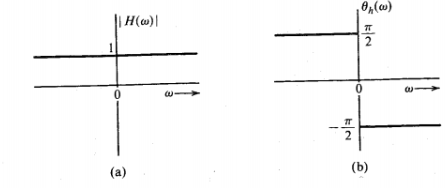
\includegraphics[]{Capture2.PNG}
	\caption{Transfer function of an ideal $\pi$/2 phase shifter(Hilbert Transformer)}
\end{figure}

It follows that if $m(t)$ is passed through a transfer function $H(\omega)=-jsgn(\omega)$, then the output is $m_h(t)$,the Hilbert Transform of $m(t)$.
Because,\newline
when $\omega>0$,

\begin{equation}
\begin{split}
H(\omega) & =-jsgn(\omega) \\
&=-j=1e^{-j\pi/2} 
\end{split}
\end{equation}

when $\omega<0$,

\begin{equation}
\begin{split}
H(\omega) & =-jsgn(\omega) \\
&=j=1e^{j\pi/2} 
\end{split}
\end{equation}

It follows that $|H(\omega)|=1$ and that $\theta_h(\omega)=-\pi/2$ for $\omega>0$ and $\pi/2$ for $\omega<0$ as shown in the above figure.Hilbert Transformer is an ideal phase shifter that shifts the phase of every spectral component by -$\pi/2$.We can now express the SSB signal in terms of $m(t)$ and $m_h(t)$.It is clear that the USB spectrum $\Phi_{USB}(\omega)$ can be expressed as,

\begin{equation}
	\Phi_{USB}(\omega)=M_+(\omega-\omega_c)+M_-(\omega+\omega_c)
\end{equation}

The inverse transform of this equation yields,

\begin{equation}
	w\phi_{USB}(t)=m_+(t)e^{j\omega_ct}+m_-(t)e^{-j\omega_ct}
\end{equation}

Substituting it in the previous equation yields,

\begin{equation}
	\phi_{USB}(t)=m(t)\cos\omega_ct-m_h(t)\sin\omega_ct
\end{equation}

Using a similar argument we can show that,

\begin{equation}
	\phi_{LSB}(t)=m(t)\cos\omega_ct+m_h(t)\sin\omega_ct
\end{equation}

Hence, a general SSB signal $\phi_{SSB}(t)$ can be expressed as,

\begin{equation}
	\phi_{SSB}(t)=m(t)\cos\omega_ct\pm m_h(t)\sin\omega_ct
\end{equation} 

\subsection{Demodulation of SSB-SC Signals}
It was shown earlier that SSB-SC signals can be coherently demodulated.We can readily varify this in another way,

\begin{equation}
\phi_{SSB}(t)=m(t)\cos\omega_ct\pm m_h(t)\sin\omega_ct
\end{equation} 

Hence,

\begin{equation}
\phi_{SSB}(t)\cos{\omega_ct}=\frac{1}{2}m(t)[1+\cos{2\omega_ct}]\pm \frac{1}{2} m_h(t) \sin{2\omega_ct} 
\end{equation}

\begin{figure}[H]
	\centering
	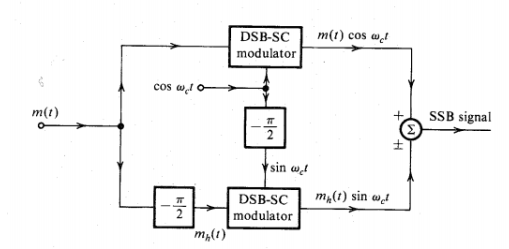
\includegraphics[]{Capture3.PNG}
	\caption{SSB Generation by Phase Shift Method}
\end{figure}


\newpage
\subsection{Envelope Detection of SSB Signals with a Carrier(SSB+C)}
We now consider SSB signals with additional carrier. Such signals can be expressed as,

\begin{equation}
	\phi_{SSB+C}=A\cos{\omega_ct}+[m(t)\cos{\omega_ct}+m_h(t)\sin{\omega_ct}]
\end{equation}

Although $m(t)$ can be recovered by synchronous detection,if A, the carrier amplitude is large enough. $m(t)$ can also be recovered from $\phi_{SSB+C}$ by envelope or rectifier detection. This can be shown by rewriting $\phi_{SSB+C}$ as

\begin{equation}
	\begin{split}
	\phi_{SSB+C} & = [A+m(t)]\cos{\omega_ct}+m_h(t)\sin{\omega_ct} \\
	& = E(t) \cos{(\omega_ct+\theta)}
	\end{split}
\end{equation}

Where $E(t)$ the envelope of $\phi_{SSB+C}$ is given by,

\begin{equation}
\begin{split}
 E(t) & =[[A+m(t)]^2 + {m_h}^2(t)]^{1/2} \\
 & = A[1+\frac{2m(t)}{A}+\frac{m^2(t)}{A^2}+\frac{m_h^2(t)}{A^2}]^{1/2}
\end{split}	
\end{equation}

If A$\gg$ $|m(t)|$, then in general A$\gg$ $m_h(t)$.Thus,

\begin{equation}
	E(t) \simeq A[1+\frac{2m(t)}{A}]^{1/2}
\end{equation}

Using binomial expression we get,

\begin{equation}
	\begin{split}
	E(t) & \simeq A[1+\frac{m(t)}{A}] \\
	& =A + m(t)
	\end{split}
\end{equation}

It is evident that for a large carrier, the SSB+C can be demodulated by an envelope detector.

In AM,envelope detection requires the condition $A\geq|m(t)|$ whereas for SSB+C, the condition is $A \gg |m(t)|$. Hence in SSB case the required carrier amplitude is much larger than that in AM,and,consequently, the efficiency of SSB+C is pathetically low.  

